\documentclass[10pt]{beamer}

\usetheme{Madrid}
\usecolortheme{default}

\usepackage{graphicx}
\usepackage{amsmath}
\usepackage{subfig}
\usepackage{textcomp}

\title[DECT-2020 NR Latency]{Measurement-Driven Latency Analysis of UL/DL Scheduling in DECT-2020 NR}

\author{
Ashuqullah Alizai \and Mohammad Reza Mousavi \and Stephan Ludwig
}

\institute{
Aalen University of Applied Sciences, Germany
}

\date{
Presented at IEEE INSECT-2026\\
Pune, India\\
29--30 May 2026
}

\begin{document}

%------------------------------------------------
\begin{frame}
\titlepage
\end{frame}

%------------------------------------------------
\begin{frame}{Motivation}
\begin{itemize}
    \item DECT-2020 NR targets low-latency private and industrial wireless networks.
    \item Existing studies mainly report end-to-end latency.
    \item The internal contribution of UL/DL scheduling and RX--TX turnaround is not well quantified.
    \item This is important for short-packet and request--response industrial traffic.
\end{itemize}

\begin{block}{Main Question}
How much latency is caused by RX--TX turnaround in practical DECT-2020 NR systems?
\end{block}
\end{frame}

%------------------------------------------------
\begin{frame}{Problem Statement and Contribution}
\begin{itemize}
    \item Single-transceiver platforms cannot transmit and receive simultaneously.
    \item Each UL/DL direction change requires hardware and firmware reconfiguration.
    \item This creates RX--TX turnaround delay.
\end{itemize}

\begin{block}{Contributions}
\begin{itemize}
    \item Measurement-based RX--TX turnaround analysis.
    \item Evaluation of sequential and grouped UL scheduling.
    \item Identification of hardware-induced latency limits.
\end{itemize}
\end{block}
\end{frame}

%------------------------------------------------
\begin{frame}{System Model}
\begin{figure}
\centering
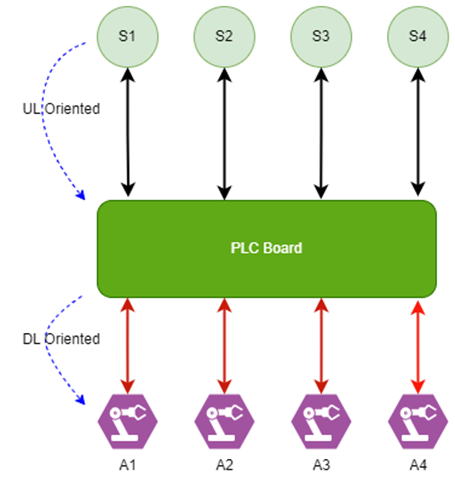
\includegraphics[width=0.78\linewidth]{SandAC.png}
\caption{Industrial sensor--actuator DECT-2020 NR star topology.}
\end{figure}
\end{frame}

%------------------------------------------------
\begin{frame}{Latency Components}
End-to-end latency is decomposed as:

\begin{equation}
L_{\mathrm{E2E}} =
L_{\mathrm{sched}} +
L_{\mathrm{turnaround}} +
L_{\mathrm{PHY}}
\end{equation}

\begin{itemize}
    \item $L_{\mathrm{sched}}$: MAC scheduling and queuing delay
    \item $L_{\mathrm{turnaround}}$: RX--TX switching delay
    \item $L_{\mathrm{PHY}}$: physical-layer transmission time
\end{itemize}

\begin{alertblock}{Focus}
This work focuses on RX--TX turnaround and scheduling impact.
\end{alertblock}
\end{frame}

%------------------------------------------------
\begin{frame}{Experimental Setup}
\begin{figure}
\centering
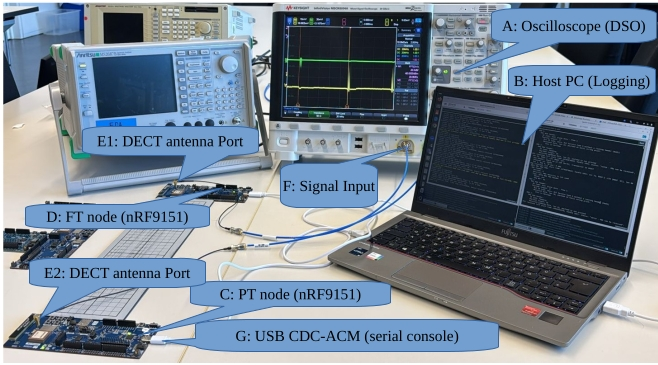
\includegraphics[width=0.82\linewidth]{main_setup.jpg}
\caption{Laboratory setup using two nRF9151 nodes and DSO measurements.}
\end{figure}

\begin{itemize}
    \item One node configured as FT, one as PT.
    \item GPIO markers capture RX completion and TX start.
\end{itemize}
\end{frame}

%------------------------------------------------
\begin{frame}{Scheduling Scenarios}
\begin{figure}
\centering
\subfloat[Sequential UL scheduling]{
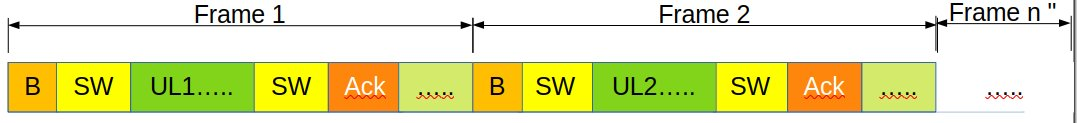
\includegraphics[width=0.47\linewidth]{scenario1.jpg}}
\hfill
\subfloat[Grouped UL scheduling]{
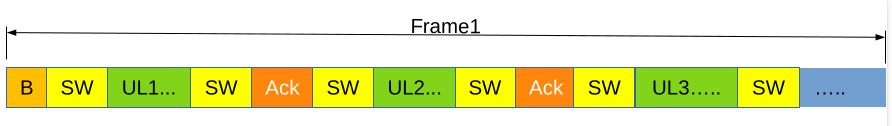
\includegraphics[width=0.47\linewidth]{scenario2.jpg}}
\caption{Evaluated UL scheduling scenarios.}
\end{figure}

\begin{itemize}
    \item Scenario 1: each UL packet followed by DL acknowledgment.
    \item Scenario 2: multiple UL packets grouped in one frame.
\end{itemize}
\end{frame}

%------------------------------------------------
\begin{frame}{Latency Models}
Sequential UL scheduling:

\begin{equation}
L_{n}^{(1)} =
\frac{7~\mathrm{slots} + T_{\mathrm{data}}^{UL_x}}
{10~\mathrm{ms}}
=
\frac{2.9~\mathrm{ms} + T_{\mathrm{data}}^{UL_x}}
{10~\mathrm{ms}}
\end{equation}

Grouped UL scheduling:

\begin{equation}
L_{n}^{(2)} =
\frac{19~\mathrm{slots} + T_{\mathrm{data}}^{UL_{1,2,3}}}
{10~\mathrm{ms}}
=
\frac{7.9~\mathrm{ms} + T_{\mathrm{data}}^{UL_{1,2,3}}}
{10~\mathrm{ms}}
\end{equation}
\end{frame}

%------------------------------------------------
\begin{frame}{Measured Scheduling Impact}
\begin{figure}
\centering
\subfloat[Scenario 1]{
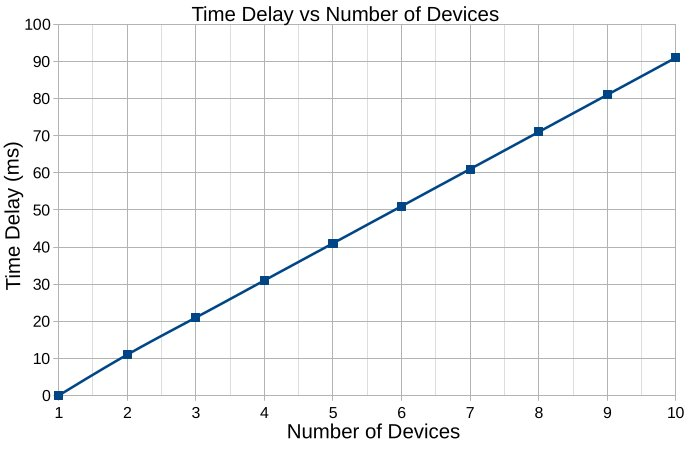
\includegraphics[width=0.47\linewidth]{s1graph.jpg}}
\hfill
\subfloat[Scenario 2]{
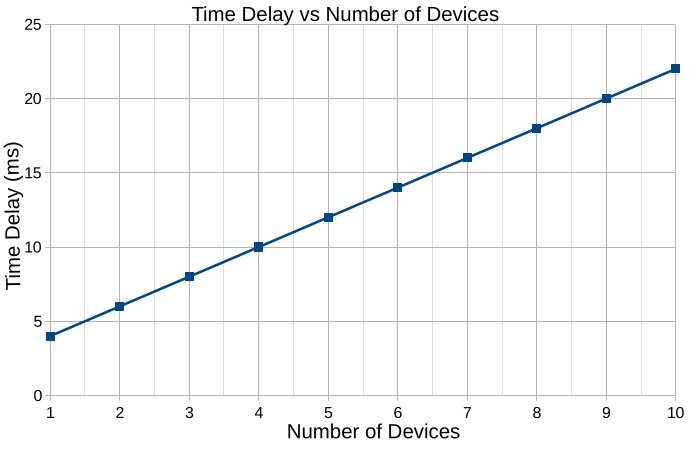
\includegraphics[width=0.47\linewidth]{s2graph.jpg}}
\caption{Measured latency versus number of UL transmissions.}
\end{figure}

\begin{itemize}
    \item Latency increases approximately linearly.
    \item Grouping reduces overhead, but does not remove turnaround delay.
\end{itemize}
\end{frame}

%------------------------------------------------
\begin{frame}{RX--TX Turnaround Measurement}
\begin{figure}
\centering
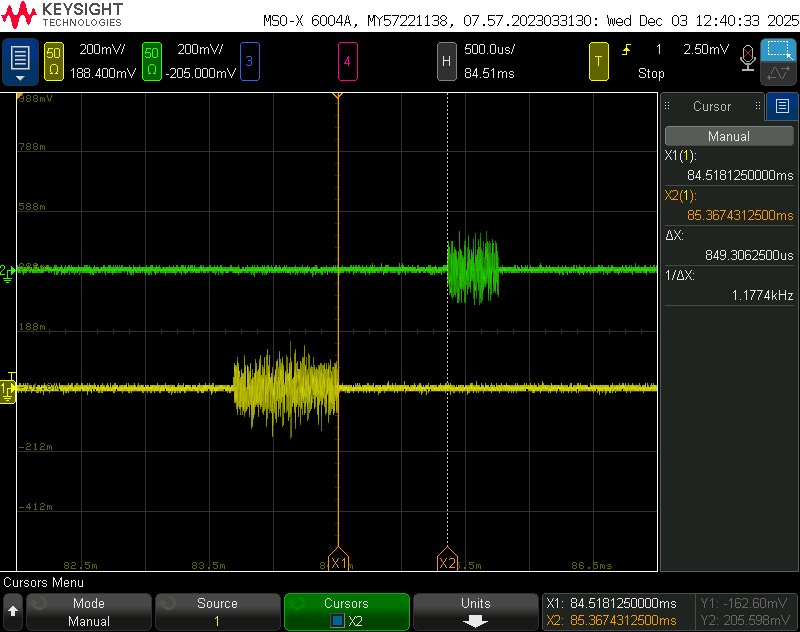
\includegraphics[width=0.78\linewidth]{osceliscope.jpg}
\caption{RX--TX turnaround measured using GPIO timing markers.}
\end{figure}

\begin{block}{Measured Result}
\[
T_{\mathrm{turnaround}} \approx 850~\mu s
\]
This corresponds to nearly two DECT-2020 NR slots.
\end{block}
\end{frame}

%------------------------------------------------
\begin{frame}{Key Findings}
\begin{itemize}
    \item RX--TX turnaround is a significant latency component.
    \item Sequential scheduling accumulates more delay due to frequent UL/DL alternation.
    \item Grouped scheduling helps, but only partially.
    \item On single-transceiver hardware, scheduling alone cannot eliminate the bottleneck.
\end{itemize}

\begin{alertblock}{Main Insight}
Latency is strongly constrained by hardware RX--TX turnaround, not only by MAC scheduling.
\end{alertblock}
\end{frame}

%------------------------------------------------
\begin{frame}{Design Implications}
\begin{itemize}
    \item Future DECT-2020 NR systems should consider:
    \begin{itemize}
        \item separate RX and TX chains,
        \item UL/DL resource separation,
        \item turnaround-aware scheduling,
        \item hybrid low-latency operating modes.
    \end{itemize}
\end{itemize}
\end{frame}

%------------------------------------------------
\begin{frame}{Conclusion}
\begin{itemize}
    \item This work presented a measurement-driven latency analysis of DECT-2020 NR.
    \item RX--TX turnaround was measured at approximately $850~\mu s$.
    \item This delay is nearly two DECT-2020 NR slots.
    \item Turnaround dominates short-packet and request--response traffic.
    \item Low-latency DECT-2020 NR design requires hardware-aware scheduling.
\end{itemize}
\end{frame}

%------------------------------------------------
\begin{frame}
\centering
\Huge Thank You\\[0.5cm]
\Large Questions?
\end{frame}

\end{document}